\documentclass{standalone}\usepackage[]{graphicx}\usepackage[]{color}
%% maxwidth is the original width if it is less than linewidth
%% otherwise use linewidth (to make sure the graphics do not exceed the margin)
\makeatletter
\def\maxwidth{ %
  \ifdim\Gin@nat@width>\linewidth
    \linewidth
  \else
    \Gin@nat@width
  \fi
}
\makeatother

\definecolor{fgcolor}{rgb}{0.345, 0.345, 0.345}
\newcommand{\hlnum}[1]{\textcolor[rgb]{0.686,0.059,0.569}{#1}}%
\newcommand{\hlstr}[1]{\textcolor[rgb]{0.192,0.494,0.8}{#1}}%
\newcommand{\hlcom}[1]{\textcolor[rgb]{0.678,0.584,0.686}{\textit{#1}}}%
\newcommand{\hlopt}[1]{\textcolor[rgb]{0,0,0}{#1}}%
\newcommand{\hlstd}[1]{\textcolor[rgb]{0.345,0.345,0.345}{#1}}%
\newcommand{\hlkwa}[1]{\textcolor[rgb]{0.161,0.373,0.58}{\textbf{#1}}}%
\newcommand{\hlkwb}[1]{\textcolor[rgb]{0.69,0.353,0.396}{#1}}%
\newcommand{\hlkwc}[1]{\textcolor[rgb]{0.333,0.667,0.333}{#1}}%
\newcommand{\hlkwd}[1]{\textcolor[rgb]{0.737,0.353,0.396}{\textbf{#1}}}%

\usepackage{framed}
\makeatletter
\newenvironment{kframe}{%
 \def\at@end@of@kframe{}%
 \ifinner\ifhmode%
  \def\at@end@of@kframe{\end{minipage}}%
  \begin{minipage}{\columnwidth}%
 \fi\fi%
 \def\FrameCommand##1{\hskip\@totalleftmargin \hskip-\fboxsep
 \colorbox{shadecolor}{##1}\hskip-\fboxsep
     % There is no \\@totalrightmargin, so:
     \hskip-\linewidth \hskip-\@totalleftmargin \hskip\columnwidth}%
 \MakeFramed {\advance\hsize-\width
   \@totalleftmargin\z@ \linewidth\hsize
   \@setminipage}}%
 {\par\unskip\endMakeFramed%
 \at@end@of@kframe}
\makeatother

\definecolor{shadecolor}{rgb}{.97, .97, .97}
\definecolor{messagecolor}{rgb}{0, 0, 0}
\definecolor{warningcolor}{rgb}{1, 0, 1}
\definecolor{errorcolor}{rgb}{1, 0, 0}
\newenvironment{knitrout}{}{} % an empty environment to be redefined in TeX

\usepackage{alltt}
\standaloneconfig{float=true}
\usepackage{tikz}
\usepackage{pgfplots}
\usepackage{fontspec}
\usepackage{caption}
\usetikzlibrary{decorations.text,pgfplots.groupplots,intersections,shapes.multipart}
\pgfplotsset{compat=1.7}

\definecolor{nice_blue}{HTML}{377EB8}
\definecolor{nice_green}{HTML}{80C87D}
\definecolor{nice_purple}{HTML}{984EA3}
\definecolor{nice_red}{HTML}{E41A1C}
\definecolor{nice_orange}{HTML}{FF7F00}
\definecolor{nice_light_orange}{HTML}{FDBF6F}
\definecolor{nice_yellow}{HTML}{FFFF99}
\definecolor{nice_pink}{HTML}{FB9A99}
\IfFileExists{upquote.sty}{\usepackage{upquote}}{}
\begin{document}

\begin{tikzpicture}

%%%%%%%%%%%%%%%%Optimal

\node (parenting_sit) at (13,6.7+3) 
  [draw
  ,circle
  ,minimum size=4cm
  ,align=center
  ,fill=nice_green
  ,line width=2.83464567pt
  ,draw=gray!80] 
  {\fontspec{Frutiger LT Std 55 Roman}Parenting \\ 
    \fontspec{Frutiger LT Std 55 Roman}Situation \\
    \emph{\fontspec{Frutiger LT Std 55 Roman}High} \\
    \emph{\fontspec{Frutiger LT Std 55 Roman}Resource Levels}};

\node[draw
      ,circle
      ,minimum width=4cm
      ,fill=nice_green
      ,line width=2.83464567pt
      ,draw=gray!80
      ] (auto_mode) at (13,3)
    {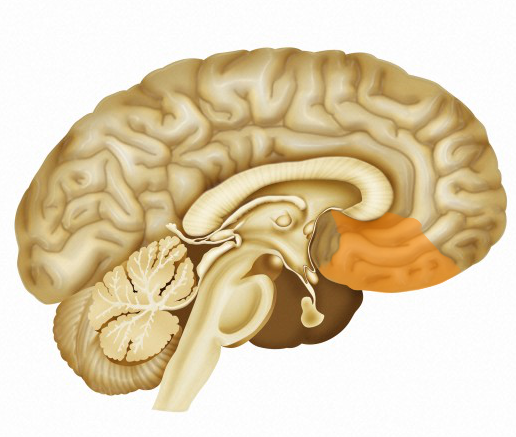
\includegraphics[width=.25\textwidth]{N0036253_mod.png}};
\node[draw=none] 
   (auto_mode_cover) at (13,1.5) {\fontspec{Frutiger LT Std 55 Roman}Automatic};

\node[draw
      ,circle
      ,minimum width=4cm
      ,fill=white
      ,line width=2.83464567pt
      ,draw=gray!80
      ,dashed
      ] (manual_mode) at (7,3)
    {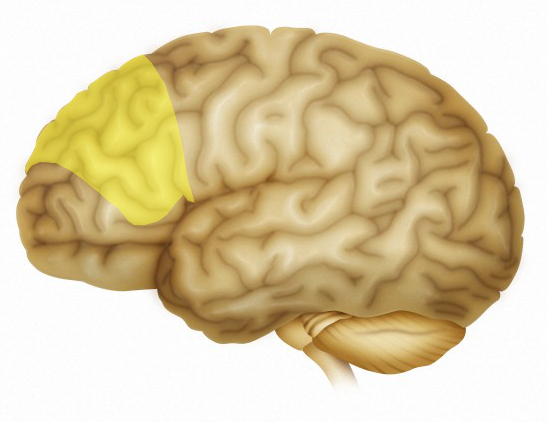
\includegraphics[width=.25\textwidth]{N0036254_mod.png}};
\node[draw=none] 
   (auto_mode_cover) at (7,1.5) {\fontspec{Frutiger LT Std 55 Roman}Manual};


% \node[circle split
%       ,draw=none
%       ,minimum width=4cm
%       ,append after command={%
%        \pgfextra{\draw (\tikzlastnode.center) -- (\tikzlastnode.south);
%                  \draw[fill=nice_green
%                       ,line width=2.83464567pt
%                       ,draw=gray!80
%                       ] (\tikzlastnode.west) arc (180:0:2cm) -- cycle;
%                  \draw[fill=nice_green
%                       ,line width=2.83464567pt
%                       ,draw=gray!80
%                       ] (\tikzlastnode.east) arc (0:180:2cm) -- cycle;
%                  \draw[fill=nice_green
%                       ,line width=2.83464567pt
%                       ,draw=gray!80
%                       ] (\tikzlastnode.center) -- (\tikzlastnode.west) arc (180:270:2cm) -- cycle;
%                  \draw[fill=white
%                       ,line width=2.83464567pt
%                       ,dashed
%                       ,draw=gray!80
%                       ] (\tikzlastnode.center) -- (\tikzlastnode.east) arc (0:-90:2cm) -- cycle;
%                 } 
%                 }
%         ]  at (13,-3.35) (parenting_beh)  {};
% \node[yshift=2em, align=center] at (parenting_beh.center) 
%   {\fontspec{Frutiger LT Std 55 Roman}Parenting \\ 
%     \fontspec{Frutiger LT Std 55 Roman}Behavior};  
% \node[xshift=-2.5em,yshift=-2.51em, align=center] at (parenting_beh.center) 
%   {\fontspec{Frutiger LT Std 55 Roman}Altruistic}; 
% \node[xshift= 2.5em,yshift=-2em, align=center] at (parenting_beh.center) 
%   {\fontspec{Frutiger LT Std 55 Roman}Non \\
%   \fontspec{Frutiger LT Std 55 Roman}Altruistic};       


\node[circle split
      ,draw=none
      ,minimum width=4cm
      ,append after command={%
       \pgfextra{\draw (\tikzlastnode.center) -- (\tikzlastnode.south);
                 \draw[fill=nice_green
                      ,line width=2.83464567pt
                      ,draw=gray!80
                      ] (\tikzlastnode.west) arc (180:0:2cm) -- cycle;
                 \draw[fill=nice_green
                      ,line width=2.83464567pt
                      ,draw=gray!80
                      ] (\tikzlastnode.east) arc (0:180:2cm) -- cycle;
                 \draw[fill=nice_green
                      ,line width=2.83464567pt
                      ,draw=gray!80
                      ] (\tikzlastnode.center) -- (\tikzlastnode.west) arc (180:270:2cm) -- cycle;
                 \draw[fill=white
                      ,line width=2.83464567pt
                      ,dashed
                      ,draw=gray!80
                      ] (\tikzlastnode.center) -- (\tikzlastnode.east) arc (0:-90:2cm) -- cycle;
                } 
                }
        ]  at (13,-3.35) (parenting_beh)  {};
\node[yshift=2em, align=center] at (parenting_beh.center) 
  {\fontspec{Frutiger LT Std 55 Roman}Parenting \\ 
    \fontspec{Frutiger LT Std 55 Roman}Behavior};  
\node[xshift=-2.5em,yshift=-2.51em, align=center] at (parenting_beh.center) 
  {\fontspec{Frutiger LT Std 55 Roman}Altruistic}; 
\node[xshift= 2.5em,yshift=-2em, align=center] at (parenting_beh.center) 
  {\fontspec{Frutiger LT Std 55 Roman}Non \\
  \fontspec{Frutiger LT Std 55 Roman}Altruistic};  


\node[circle split
      ,draw=none
      ,minimum width=4cm,
      ,append after command={%
       \pgfextra{\draw (\tikzlastnode.center) -- (\tikzlastnode.south);
                 \draw[fill=nice_green
                      ,line width=2.83464567pt
                      ,draw=gray!80
                      ] (\tikzlastnode.west) arc (180:0:2cm) -- cycle;
                 \draw[fill=nice_green
                      ,line width=2.83464567pt
                      ,draw=gray!80
                      ] (\tikzlastnode.east) arc (0:180:2cm) -- cycle;
                 \draw[fill=nice_green
                      ,line width=2.83464567pt
                      ,draw=gray!80] (\tikzlastnode.center) -- (\tikzlastnode.west) arc (180:270:2cm) -- cycle;
                 \draw[fill=white
                      ,dashed
                      ,line width=2.83464567pt
                      ,draw=gray!80] (\tikzlastnode.center) -- (\tikzlastnode.east) arc (0:-90:2cm) -- cycle;
                } 
                }
        ] at (13,-3.35-6.7) (child_wb)  {};
\node[yshift=2em, align=center] at (child_wb.center) 
  {\fontspec{Frutiger LT Std 55 Roman}Child \\ 
    \fontspec{Frutiger LT Std 55 Roman}Wellbeing};  
\node[xshift=-2.5em,yshift=-1.955em, align=center] at (child_wb.center) 
  {\textbf{\fontspec{Frutiger LT Std 55 Roman}\char"2265} \\
  \fontspec{Frutiger LT Std 55 Roman}Threshold}; 
\node[xshift= 2.5em,yshift=-2em, align=center] at (child_wb.center) 
  {\fontspec{Frutiger LT Std 55 Roman} < \\
  \fontspec{Frutiger LT Std 55 Roman}Threshold};   

\draw[->,line width=2.83464567pt,draw=gray!80]  
  (parenting_sit) to node [auto] {} (auto_mode);
  
\draw[->,line width=2.83464567pt,draw=gray!80]  
  (auto_mode) to node [auto] {} (parenting_beh);  
  
\draw[->,line width=2.83464567pt, align=center, draw=gray!80, dashed, bend right]  
  (auto_mode) to node [above=40pt, auto] 
    {\fontspec{Frutiger LT Std 55 Roman}Manual Mode \\
    \fontspec{Frutiger LT Std 55 Roman}Transition (Tx)} 
  (manual_mode);  

\draw[->,line width=2.83464567pt, bend right, draw=gray!80, dashed]  
  (manual_mode) to node [auto] {} (parenting_beh);  

\draw[->,line width=2.83464567pt,draw=gray!80]  
  (parenting_beh) to node [auto] {} (child_wb);
  
%%%%%Suboptimal

\node (parenting_sit_sub) at (13*2,6.7+3) 
  [draw
  ,circle
  ,minimum size=4cm
  ,align=center
  ,fill=nice_light_orange
  ,line width=2.83464567pt
  ,draw=gray!80] 
  {\fontspec{Frutiger LT Std 55 Roman}Parenting \\ 
    \fontspec{Frutiger LT Std 55 Roman}Situation \\
    \emph{\fontspec{Frutiger LT Std 55 Roman}Moderate} \\
    \emph{\fontspec{Frutiger LT Std 55 Roman}Resource Levels}};

\node[draw
      ,circle
      ,minimum width=4cm
      ,fill=nice_light_orange
      ,line width=2.83464567pt
      ,draw=gray!80
      ] (auto_mode_sub) at (13*2,3)
    {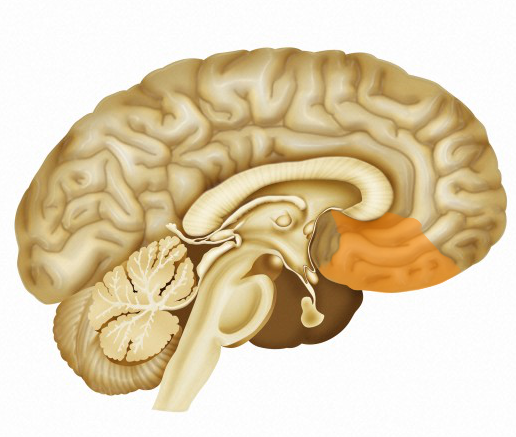
\includegraphics[width=.25\textwidth]{N0036253_mod.png}};
\node[draw=none] 
   (auto_mode_cover_sub) at (13*2,1.5) {\fontspec{Frutiger LT Std 55 Roman}Automatic};

\node[draw
      ,circle
      ,minimum width=4cm
      ,fill=nice_light_orange
      ,line width=2.83464567pt
      ,draw=gray!80
      ] (manual_mode_sub) at (7+13,3)
    {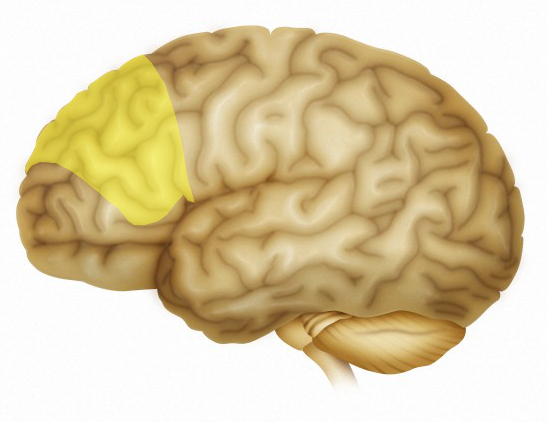
\includegraphics[width=.25\textwidth]{N0036254_mod.png}};
\node[draw=none] 
   (manual_mode_cover_sub) at (7+13,1.5) {\fontspec{Frutiger LT Std 55 Roman}Manual};


\node[circle split
      ,draw=none
      ,minimum width=4cm
      ,append after command={%
       \pgfextra{\draw (\tikzlastnode.center) -- (\tikzlastnode.south);
                 \draw[fill=nice_light_orange
                      ,line width=2.83464567pt
                      ,draw=gray!80
                      ] (\tikzlastnode.west) arc (180:0:2cm) -- cycle;
                 \draw[fill=nice_light_orange
                      ,line width=2.83464567pt
                      ,draw=gray!80
                      ] (\tikzlastnode.east) arc (0:180:2cm) -- cycle;
                 \draw[fill=nice_light_orange
                      ,line width=2.83464567pt
                      ,draw=gray!80
                      ] (\tikzlastnode.center) -- (\tikzlastnode.west) arc (180:270:2cm) -- cycle;
                 \draw[fill=white
                      ,line width=2.83464567pt
                      ,draw=gray!80
                      ,dashed
                      ] (\tikzlastnode.center) -- (\tikzlastnode.east) arc (0:-90:2cm) -- cycle;
                } 
                }
        ]  at (13*2,-3.35) (parenting_beh_sub)  {};
\node[yshift=2em, align=center] at (parenting_beh_sub.center) 
  {\fontspec{Frutiger LT Std 55 Roman}Parenting \\ 
    \fontspec{Frutiger LT Std 55 Roman}Behavior};  
\node[xshift=-2.5em,yshift=-2.51em, align=center] at (parenting_beh_sub.center) 
  {\fontspec{Frutiger LT Std 55 Roman}Altruistic}; 
\node[xshift= 2.5em,yshift=-2em, align=center] at (parenting_beh_sub.center) 
  {\fontspec{Frutiger LT Std 55 Roman}Non \\
  \fontspec{Frutiger LT Std 55 Roman}Altruistic};       

\node[circle split
      ,draw=none
      ,minimum width=4cm,
      ,append after command={%
       \pgfextra{\draw (\tikzlastnode.center) -- (\tikzlastnode.south);
                 \draw[fill=nice_light_orange
                      ,line width=2.83464567pt
                      ,draw=gray!80
                      ] (\tikzlastnode.west) arc (180:0:2cm) -- cycle;
                 \draw[fill=nice_light_orange
                      ,line width=2.83464567pt
                      ,draw=gray!80
                      ] (\tikzlastnode.east) arc (0:180:2cm) -- cycle;
                 \draw[fill=nice_light_orange
                      ,line width=2.83464567pt
                      ,draw=gray!80] (\tikzlastnode.center) -- (\tikzlastnode.west) arc (180:270:2cm) -- cycle;
                 \draw[fill=white
                      ,line width=2.83464567pt
                      ,dashed
                      ,draw=gray!80] (\tikzlastnode.center) -- (\tikzlastnode.east) arc (0:-90:2cm) -- cycle;
                } 
                }
        ] at (13*2,-3.35-6.7) (child_wb_sub)  {};
\node[yshift=2em, align=center] at (child_wb_sub.center) 
  {\fontspec{Frutiger LT Std 55 Roman}Child \\ 
    \fontspec{Frutiger LT Std 55 Roman}Wellbeing};  
\node[xshift=-2.5em,yshift=-1.955em, align=center] at (child_wb_sub.center) 
  {\textbf{\fontspec{Frutiger LT Std 55 Roman}\char"2265} \\
  \fontspec{Frutiger LT Std 55 Roman}Threshold}; 
\node[xshift= 2.5em,yshift=-2em, align=center] at (child_wb_sub.center) 
  {\fontspec{Frutiger LT Std 55 Roman} < \\
  \fontspec{Frutiger LT Std 55 Roman}Threshold};   

\draw[->,line width=2.83464567pt,draw=gray!80]  
  (parenting_sit_sub) to node [auto] {} (auto_mode_sub);
  
\draw[->,line width=2.83464567pt,draw=gray!80, dashed]  
  (auto_mode_sub) to node [auto] {} (parenting_beh_sub);  
  
\draw[->,line width=2.83464567pt, align=center, draw=gray!80, bend right]  
  (auto_mode_sub) to node [above=40pt, auto] 
    {\fontspec{Frutiger LT Std 55 Roman}Manual Mode \\
    \fontspec{Frutiger LT Std 55 Roman}Transition (Tx)} 
  (manual_mode_sub);  

\draw[->,line width=2.83464567pt, bend right, draw=gray!80]  
  (manual_mode_sub) to node [auto] {} (parenting_beh_sub);  

\draw[->,line width=2.83464567pt,draw=gray!80]  
  (parenting_beh_sub) to node [auto] {} (child_wb_sub);


%%%%%Constrained

\node (parenting_sit_con) at (13*3,6.7+3) 
  [draw
  ,circle
  ,minimum size=4cm
  ,align=center
  ,fill=nice_pink
  ,line width=2.83464567pt
  ,draw=gray!80] 
  {\fontspec{Frutiger LT Std 55 Roman}Parenting \\ 
    \fontspec{Frutiger LT Std 55 Roman}Situation \\
    \emph{\fontspec{Frutiger LT Std 55 Roman}Low} \\
    \emph{\fontspec{Frutiger LT Std 55 Roman}Resource Levels}};

\node[draw
      ,circle
      ,minimum width=4cm
      ,fill=nice_pink
      ,line width=2.83464567pt
      ,draw=gray!80
      ] (auto_mode_con) at (13*3,3)
    {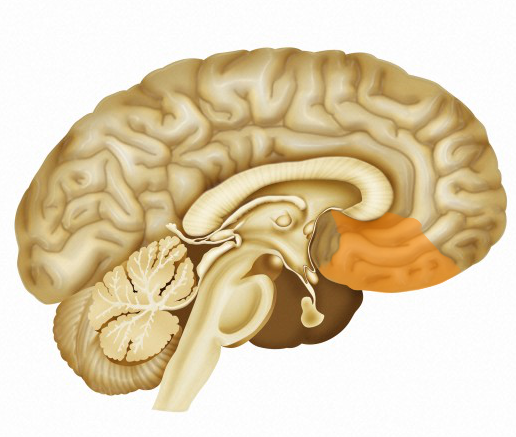
\includegraphics[width=.25\textwidth]{N0036253_mod.png}};
\node[draw=none] 
   (auto_mode_cover_con) at (13*3,1.5) {\fontspec{Frutiger LT Std 55 Roman}Automatic};

\node[draw
      ,dashed
      ,circle
      ,minimum width=4cm
      ,fill=white
      ,line width=2.83464567pt
      ,draw=gray!80
      ] (manual_mode_con) at (7+13*2,3)
    {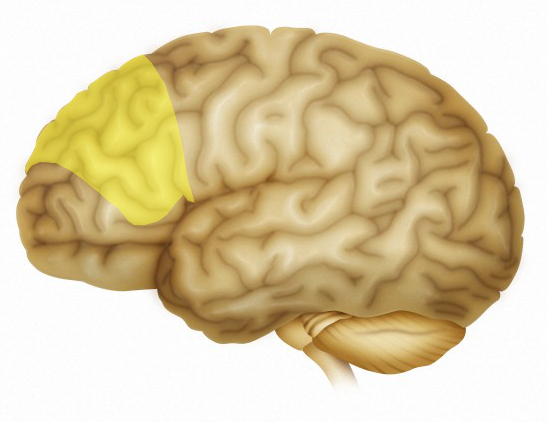
\includegraphics[width=.25\textwidth]{N0036254_mod.png}};
\node[draw=none] 
   (manual_mode_cover_con) at (7+13*2,1.5) {\fontspec{Frutiger LT Std 55 Roman}Manual};


\node[circle split
      ,draw=none
      ,minimum width=4cm
      ,append after command={%
       \pgfextra{\draw (\tikzlastnode.center) -- (\tikzlastnode.south);
                 \draw[fill=nice_pink
                      ,line width=2.83464567pt
                      ,draw=gray!80
                      ] (\tikzlastnode.west) arc (180:0:2cm) -- cycle;
                 \draw[fill=nice_pink
                      ,line width=2.83464567pt
                      ,draw=gray!80
                      ] (\tikzlastnode.east) arc (0:180:2cm) -- cycle;
                 \draw[fill=white
                      ,dashed
                      ,line width=2.83464567pt
                      ,draw=gray!80] (\tikzlastnode.center) -- (\tikzlastnode.west) arc (180:270:2cm) -- cycle;
                 \draw[fill=white
                      ,line width=2.83464567pt
                      ,nice_pink
                      ,draw=gray!80] (\tikzlastnode.center) -- (\tikzlastnode.east) arc (0:-90:2cm) -- cycle;
                } 
                }
        ]  at (13*3,-3.35) (parenting_beh_con)  {};
\node[yshift=2em, align=center] at (parenting_beh_con.center) 
  {\fontspec{Frutiger LT Std 55 Roman}Parenting \\ 
    \fontspec{Frutiger LT Std 55 Roman}Behavior};  
\node[xshift=-2.5em,yshift=-2.51em, align=center] at (parenting_beh_con.center) 
  {\fontspec{Frutiger LT Std 55 Roman}Altruistic}; 
\node[xshift= 2.5em,yshift=-2em, align=center] at (parenting_beh_con.center) 
  {\fontspec{Frutiger LT Std 55 Roman}Non \\
  \fontspec{Frutiger LT Std 55 Roman}Altruistic};       

\node[circle split
      ,draw=none
      ,minimum width=4cm,
      ,append after command={%
       \pgfextra{\draw (\tikzlastnode.center) -- (\tikzlastnode.south);
                 \draw[fill=nice_pink
                      ,line width=2.83464567pt
                      ,draw=gray!80
                      ] (\tikzlastnode.west) arc (180:0:2cm) -- cycle;
                 \draw[fill=nice_pink
                      ,line width=2.83464567pt
                      ,draw=gray!80
                      ] (\tikzlastnode.east) arc (0:180:2cm) -- cycle;
                 \draw[fill=white
                      ,dashed
                      ,line width=2.83464567pt
                      ,draw=gray!80] (\tikzlastnode.center) -- (\tikzlastnode.west) arc (180:270:2cm) -- cycle;
                 \draw[fill=white
                      ,line width=2.83464567pt
                      ,nice_pink
                      ,draw=gray!80] (\tikzlastnode.center) -- (\tikzlastnode.east) arc (0:-90:2cm) -- cycle;
                } 
                }
        ] at (13*3,-3.35-6.7) (child_wb_con)  {};
\node[yshift=2em, align=center] at (child_wb_con.center) 
  {\fontspec{Frutiger LT Std 55 Roman}Child \\ 
    \fontspec{Frutiger LT Std 55 Roman}Wellbeing};  
\node[xshift=-2.5em,yshift=-1.955em, align=center] at (child_wb_con.center) 
  {\textbf{\fontspec{Frutiger LT Std 55 Roman}\char"2265} \\
  \fontspec{Frutiger LT Std 55 Roman}Threshold}; 
\node[xshift= 2.5em,yshift=-2em, align=center] at (child_wb_con.center) 
  {\fontspec{Frutiger LT Std 55 Roman} < \\
  \fontspec{Frutiger LT Std 55 Roman}Threshold};   

\draw[->,line width=2.83464567pt,draw=gray!80]  
  (parenting_sit_con) to node [auto] {} (auto_mode_con);
  
\draw[->,line width=2.83464567pt,draw=gray!80]  
  (auto_mode_con) to node [auto] {} (parenting_beh_con);  
  
\draw[->,line width=2.83464567pt, align=center, draw=gray!80, bend right, dashed]  
  (auto_mode_con) to node [above=40pt, auto] 
    {\fontspec{Frutiger LT Std 55 Roman}Manual Mode \\
    \fontspec{Frutiger LT Std 55 Roman}Transition (Tx)} 
  (manual_mode_con);  

\draw[->,line width=2.83464567pt, bend right, draw=gray!80, dashed]  
  (manual_mode_con) to node [auto] {} (parenting_beh_con);  

\draw[->,line width=2.83464567pt,draw=gray!80]  
  (parenting_beh_con) to node [auto] {} (child_wb_con);


\node[below left=1mm] at (11,-3.35-2.6) {\fbox{
\begin{tabular}{@{}r@{ }l@{}}
 \raisebox{3pt}{\tikz{\draw[line width=2.83464567pt, draw=gray!80, dashed] (0,0) -- (5mm,0);}}&
  \fontspec{Frutiger LT Std 55 Roman}Low Probability Path or Outcome\\
 \raisebox{3pt}{\tikz{\draw[line width=2.83464567pt, draw=gray!80] (0,0) -- (5mm,0);}}&
  \fontspec{Frutiger LT Std 55 Roman}High Probability Path or Outcome\\
\end{tabular}}};

\end{tikzpicture}


\end{document}
